\documentclass{article}

\usepackage{graphicx}

\graphicspath{./}
    
\begin{document}
    \title  { \textbf{SYSC 4602 Assignment 1} }
    \author {
        David Song (101071234)\\
        Ghassan Arnouk (101078550)\\
        Zachary Porter (101069001)
    }
     
    \maketitle
    
    \clearpage
    \section*{Part 3: Ethernet Frame Structure}
    \begin{figure}[htbp]
        \centering
        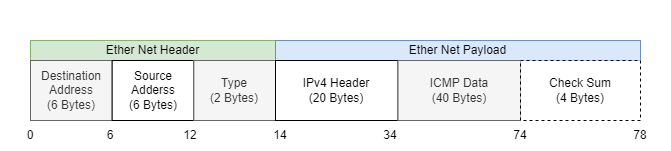
\includegraphics[width=\textwidth]{images/assignment3-part3.drawio.png}
        \caption{Ethernet Frame Structure Diagram}
    \end{figure}
    \section*{Part 4: Protocol Overhead}
    \begin{figure}[htbp]
        \centering
        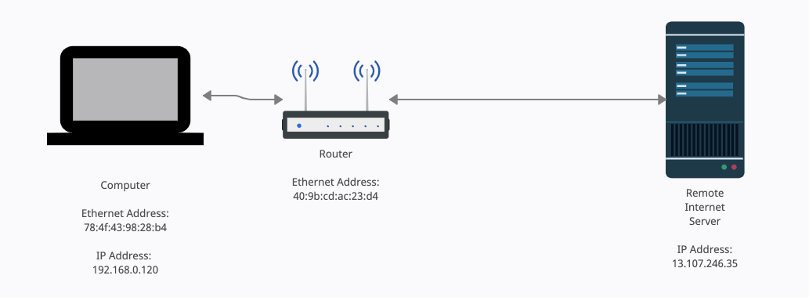
\includegraphics[width=\linewidth]{images/part4.png}
        \caption{Relative positions of computer, router, and internet server}
    \end{figure}
    \section*{Part 5: Demultiplexing Keys}
    \subsection*{What is the broadcast Ethernet address, written standard form as Wireshark displays it?}
    The broadcast ethernet address is {\bfseries FF FF FF FF FF FF} which is represented as all {\bfseries 1's} in hexadecimal.
    As stated in the lab manual, broadcast traffic is sent to a reserved Ethernet address that has all bits set to {\bfseries 1's}.
    \clearpage
    \subsection*{Which bit of the Ethernet address is used to determine whether it is unicast or multicast/broadcast?}
    The ethernet address uses the {\bfseries first bit} to determine whether it is unicast or multicast/broadcast.
    If the first bit is `0', it is denoted as unicast, whereas if it's `1', it is denoted as multicast/broadcast. 
    Note that broadcast is a special case of multicast and thus; they are both denoted using the first bit as `1'.
    \section*{Explore on your own (IEEE 802.3)}
    \subsection*{How long are the combined IEEE 802.3 and LLC headers compared to the DIX Ethernet headers?
    You can use Wireshark to work this out. Note that the Trailer/Padding and Checksum may be shown as part of the header, but they come at the end of the frame}
    \begin{itemize}
        \item IEEE 802.3 has {\bfseries 22 bytes}
        \item Logical-Link Control (LLC) has {\bfseries 3 bytes}
        \item DIX Ethernet headers have {\bfseries 14 bytes}
        \item Padding has {\bfseries 8 bytes} consisting of all zeros
    \end{itemize}
    \subsection*{How does the receiving computer know whether the frame is DIX Ethernet or IEEE 802.3? Hint: you may need to both use Wireshark to look at packet examples and read your text near where the Ethernet formats are described}
    To differentiate between DIX ethernet and IEEE 802.3, we look at the value of the type/length fields, which exist in the same position for both protocols.
    If the value is less than 0x600, then it interrupted as frame length (IEEE 802.3), otherwise it is greater than the value, therefore it is ``Type" value (DIX header).
    \subsection*{If IEEE 802.3 has no Type field, then how is the next higher layer determined? Use Wireshark to look for the demultiplexing key}
    IEEE 802.3 uses the LLC header after the IEEE 802.3 header to tell us the next higher layer protocol.
    LLC uses a single byte called Destination Service Access Point (DSAP) compared to DIX ethernet that uses 2 bytes in the Type field to denote the next protocol.
\end{document}
